\documentclass{beamer}
\mode<presentation>
\usepackage{amsmath}
\usepackage{amssymb}
%\usepackage{advdate}
\usepackage{adjustbox}
\usepackage{subcaption}
\usepackage{enumitem}
\usepackage{multicol}
\usepackage{mathtools}
\usepackage{listings}
\usepackage{float}
\usepackage{graphicx}
\usepackage{url}
\def\UrlBreaks{\do\/\do-}
\usetheme{Boadilla}
\usecolortheme{lily}
\setbeamertemplate{footline}
{
  \leavevmode%
  \hbox{%
  \begin{beamercolorbox}[wd=\paperwidth,ht=2.25ex,dp=1ex,right]{author in head/foot}%
    \insertframenumber{} / \inserttotalframenumber\hspace*{2ex} 
  \end{beamercolorbox}}%
  \vskip0pt%
}
\setbeamertemplate{navigation symbols}{}

\providecommand{\nCr}[2]{\,^{#1}C_{#2}} % nCr
\providecommand{\nPr}[2]{\,^{#1}P_{#2}} % nPr
\providecommand{\mbf}{\mathbf}
\providecommand{\pr}[1]{\ensuremath{\Pr\left(#1\right)}}
\providecommand{\qfunc}[1]{\ensuremath{Q\left(#1\right)}}
\providecommand{\sbrak}[1]{\ensuremath{{}\left[#1\right]}}
\providecommand{\lsbrak}[1]{\ensuremath{{}\left[#1\right.}}
\providecommand{\rsbrak}[1]{\ensuremath{{}\left.#1\right]}}
\providecommand{\brak}[1]{\ensuremath{\left(#1\right)}}
\providecommand{\lbrak}[1]{\ensuremath{\left(#1\right.}}
\providecommand{\rbrak}[1]{\ensuremath{\left.#1\right)}}
\providecommand{\cbrak}[1]{\ensuremath{\left\{#1\right\}}}
\providecommand{\lcbrak}[1]{\ensuremath{\left\{#1\right.}}
\providecommand{\rcbrak}[1]{\ensuremath{\left.#1\right\}}}
\theoremstyle{remark}
\newtheorem{rem}{Remark}
\newcommand{\sgn}{\mathop{\mathrm{sgn}}}
\providecommand{\abs}[1]{\left\vert#1\right\vert}
\providecommand{\res}[1]{\Res\displaylimits_{#1}} 
\providecommand{\norm}[1]{\lVert#1\rVert}
\providecommand{\mtx}[1]{\mathbf{#1}}
\providecommand{\mean}[1]{E\left[ #1 \right]}
\providecommand{\fourier}{\overset{\mathcal{F}}{ \rightleftharpoons}}
%\providecommand{\hilbert}{\overset{\mathcal{H}}{ \rightleftharpoons}}
\providecommand{\system}{\overset{\mathcal{H}}{ \longleftrightarrow}}
	%\newcommand{\solution}[2]{\textbf{Solution:}{#1}}
%\newcommand{\solution}{\noindent \textbf{Solution: }}
\providecommand{\dec}[2]{\ensuremath{\overset{#1}{\underset{#2}{\gtrless}}}}
\newcommand{\myvec}[1]{\ensuremath{\begin{pmatrix}#1\end{pmatrix}}}
\let\vec\mathbf

\lstset{
language=C,
frame=single, 
breaklines=true,
columns=fullflexible
}

\numberwithin{equation}{section}

\title{Presentation - Matgeo}
\author{Aryansingh Sonaye \\
AI25BTECH11032 \\
EE1030 - Matrix Theory}

\date{\today} 
\begin{document}

\begin{frame}
\titlepage
\end{frame}

\section{Problem}
\begin{frame}
\frametitle{Problem Statement}
Find the angle between the following pairs of lines:

\begin{enumerate}
\item[(a)] 
$\vec{r} = 2\hat i - 5\hat j + \hat k + \lambda(3\hat i + 2\hat j + 6\hat k), 
\quad
\vec{r} = 7\hat i - 6\hat j + \mu(\hat i + 2\hat j + 2\hat k)$

\item[(b)] 
$\vec{r} = 3\hat i + \hat j - 2\hat k + \lambda(\hat i - \hat j - 2\hat k), 
\quad 
\vec{r} = 2\hat i - \hat j - 5\hat k + \mu(3\hat i - 5\hat j - 4\hat k)$

\item[(c)] 
$\dfrac{x-2}{2} = \dfrac{y-1}{5} = \dfrac{z+3}{-3}, 
\quad 
\dfrac{x+2}{-1} = \dfrac{y-4}{8} = \dfrac{z-5}{-4}$

\item[(d)] 
$\dfrac{x}{2} = \dfrac{y}{5} = \dfrac{z}{1}, 
\quad 
\dfrac{x-5}{4} = \dfrac{y-2}{1} = \dfrac{z-3}{8}$
\end{enumerate}

\end{frame}

\section{Solution}
\subsection{Description of Variables used}
\begin{frame}
\frametitle{Description of Variables used}
\begin{table}[H]
\centering
\begin{tabular}{|c|c|c|c|c|}
\hline
Case & $\vec{a_1}$ & $\vec{d_1}$ & $\vec{a_2}$ & $\vec{d_2}$ \\
\hline
(a) & $\myvec{2 \\ -5 \\ 1}$ & $\myvec{3 \\ 2 \\ 6}$ & $\myvec{7 \\ -6 \\ 0}$ & $\myvec{1 \\ 2 \\ 2}$ \\
\hline
(b) & $\myvec{3 \\ 1 \\ -2}$ & $\myvec{1 \\ -1 \\ -2}$ & $\myvec{2 \\ -1 \\ -5}$ & $\myvec{3 \\ -5 \\ -4}$ \\
\hline
(c) & $\myvec{2 \\ 1 \\ -3}$ & $\myvec{2 \\ 5 \\ -3}$ & $\myvec{-2 \\ 4 \\ 5}$ & $\myvec{-1 \\ 8 \\ -4}$ \\
\hline
(d) & $\myvec{0 \\ 0 \\ 0}$ & $\myvec{2 \\ 5 \\ 1}$ & $\myvec{5 \\ 2 \\ 3}$ & $\myvec{4 \\ 1 \\ 8}$ \\
\hline
\end{tabular}
\caption{Points and direction vectors for Problem 2.2.25}
\label{}
\end{table}



\end{frame}

\subsection{Theoretical Solution }
\begin{frame}
\frametitle{Theoretical Solution}
\textbf{General Formula:}  

If two lines are given in vector form, their direction vectors are denoted as
$$
\vec{d_1}, \quad \vec{d_2}.
$$
The angle $\theta$ between the lines is the angle between these two vectors, given by
\begin{align}
\cos \theta &= \frac{\vec{d_1}^T \vec{d_2}}{\|\vec{d_1}\| \, \|\vec{d_2}\|}.
\end{align}
Here:
\begin{itemize}
    \item $\vec{d_1}, \vec{d_2}$ are the direction vectors of the given lines,
    \item $\vec{d_1}^T \vec{d_2}$ is the matrix product (dot product),
    \item $\|\vec{d_i}\| = \sqrt{\vec{d_i}^T \vec{d_i}}$ is the magnitude (norm) of vector $\vec{d_i}$.
\end{itemize}

\end{frame}

\begin{frame}
\frametitle{Theoretical Solution}
\begin{enumerate}
\item[(a)] 
$\vec{r} = 2\hat i - 5\hat j + \hat k + \lambda(3\hat i + 2\hat j + 6\hat k), 
\quad
\vec{r} = 7\hat i - 6\hat j + \mu(\hat i + 2\hat j + 2\hat k)$

\textbf{Solution:}  

\begin{align}
\vec{d_1} &= \myvec{3 \\ 2 \\ 6}, &
\vec{d_2} &= \myvec{1 \\ 2 \\ 2} \\[6pt]
\vec{d_1}^T \vec{d_2} &= \myvec{3 & 2 & 6}\myvec{1 \\ 2 \\ 2} = 19 \\[6pt]
\|\vec{d_1}\| &= \sqrt{\vec{d_1}^T \vec{d_1}} = \sqrt{49} = 7, &
\|\vec{d_2}\| &= \sqrt{\vec{d_2}^T \vec{d_2}} = \sqrt{9} = 3 \\[6pt]
\cos\theta &= \frac{19}{21}
\end{align}

\textbf{Final Answer:}  
\begin{align}
\theta &= \cos^{-1}\!\left(\tfrac{19}{21}\right)
\end{align}

\end{enumerate}

\end{frame}

\begin{frame}
\frametitle{Theoretical Solution}
\begin{enumerate}
\item[(b)] 
$\vec{r} = 3\hat i + \hat j - 2\hat k + \lambda(\hat i - \hat j - 2\hat k), 
\quad 
\vec{r} = 2\hat i - \hat j - 5\hat k + \mu(3\hat i - 5\hat j - 4\hat k)$

\textbf{Solution:}  

\begin{align}
\vec{d_1} &= \myvec{1 \\ -1 \\ -2}, &
\vec{d_2} &= \myvec{3 \\ -5 \\ -4} \\[6pt]
\vec{d_1}^T \vec{d_2} &= \myvec{1 & -1 & -2}\myvec{3 \\ -5 \\ -4} = 16 \\[6pt]
\|\vec{d_1}\| &= \sqrt{\vec{d_1}^T \vec{d_1}} = \sqrt{6}, &
\|\vec{d_2}\| &= \sqrt{\vec{d_2}^T \vec{d_2}} = \sqrt{50} \\[6pt]
\cos\theta &= \frac{16}{\sqrt{6}\cdot \sqrt{50}} = \frac{8}{5\sqrt{3}}
\end{align}
\end{enumerate}
\end{frame}

\begin{frame}
\frametitle{Theoretical Solution}

\begin{enumerate}
\item[] 
\textbf{Final Answer:}  
\begin{align}
\theta &= \cos^{-1}\!\left(\tfrac{8}{5\sqrt{3}}\right)
\end{align}


\item[(c)] 
$\dfrac{x-2}{2} = \dfrac{y-1}{5} = \dfrac{z+3}{-3}, 
\quad 
\dfrac{x+2}{-1} = \dfrac{y-4}{8} = \dfrac{z-5}{-4}$

\textbf{Solution:}  

\begin{align}
\vec{d_1} &= \myvec{2 \\ 5 \\ -3}, &
\vec{d_2} &= \myvec{-1 \\ 8 \\ -4} \\[6pt]
\vec{d_1}^T \vec{d_2} &= \myvec{2 & 5 & -3}\myvec{-1 \\ 8 \\ -4} = 50 \\[6pt]
\|\vec{d_1}\| &= \sqrt{\vec{d_1}^T \vec{d_1}} = \sqrt{38}, &
\|\vec{d_2}\| &= \sqrt{\vec{d_2}^T \vec{d_2}} = 9
\end{align}
\end{enumerate}

\end{frame}

\begin{frame}
\frametitle{Theoretical Solution}
\begin{enumerate}
\item[]
\begin{align}
\cos\theta &= \frac{50}{9\sqrt{38}}
\end{align}

\textbf{Final Answer:}  
\begin{align}
\theta &= \cos^{-1}\!\left(\tfrac{50}{9\sqrt{38}}\right)
\end{align}

\item[(d)] 
$\dfrac{x}{2} = \dfrac{y}{5} = \dfrac{z}{1}, 
\quad 
\dfrac{x-5}{4} = \dfrac{y-2}{1} = \dfrac{z-3}{8}$

\end{enumerate}
    
\end{frame}

\begin{frame}
\frametitle{Theoretical Solution}

\begin{enumerate}
\item[]
\textbf{Solution:}  

\begin{align}
\vec{d_1} &= \myvec{2 \\ 5 \\ 1}, &
\vec{d_2} &= \myvec{4 \\ 1 \\ 8} \\[6pt]
\vec{d_1}^T \vec{d_2} &= \myvec{2 & 5 & 1}\myvec{4 \\ 1 \\ 8} = 21 \\[6pt]
\|\vec{d_1}\| &= \sqrt{\vec{d_1}^T \vec{d_1}} = \sqrt{30}, &
\|\vec{d_2}\| &= \sqrt{\vec{d_2}^T \vec{d_2}} = 9 \\[6pt]
\cos\theta &= \frac{21}{9\sqrt{30}} = \frac{7}{3\sqrt{30}}
\end{align}

\textbf{Final Answer:}  
\begin{align}
\theta &= \cos^{-1}\!\left(\tfrac{7}{3\sqrt{30}}\right)
\end{align}

\end{enumerate}
    
\end{frame}


\subsection{Plot}
\begin{frame}
    \frametitle{Plot}
\begin{figure}[H]
    \centering
    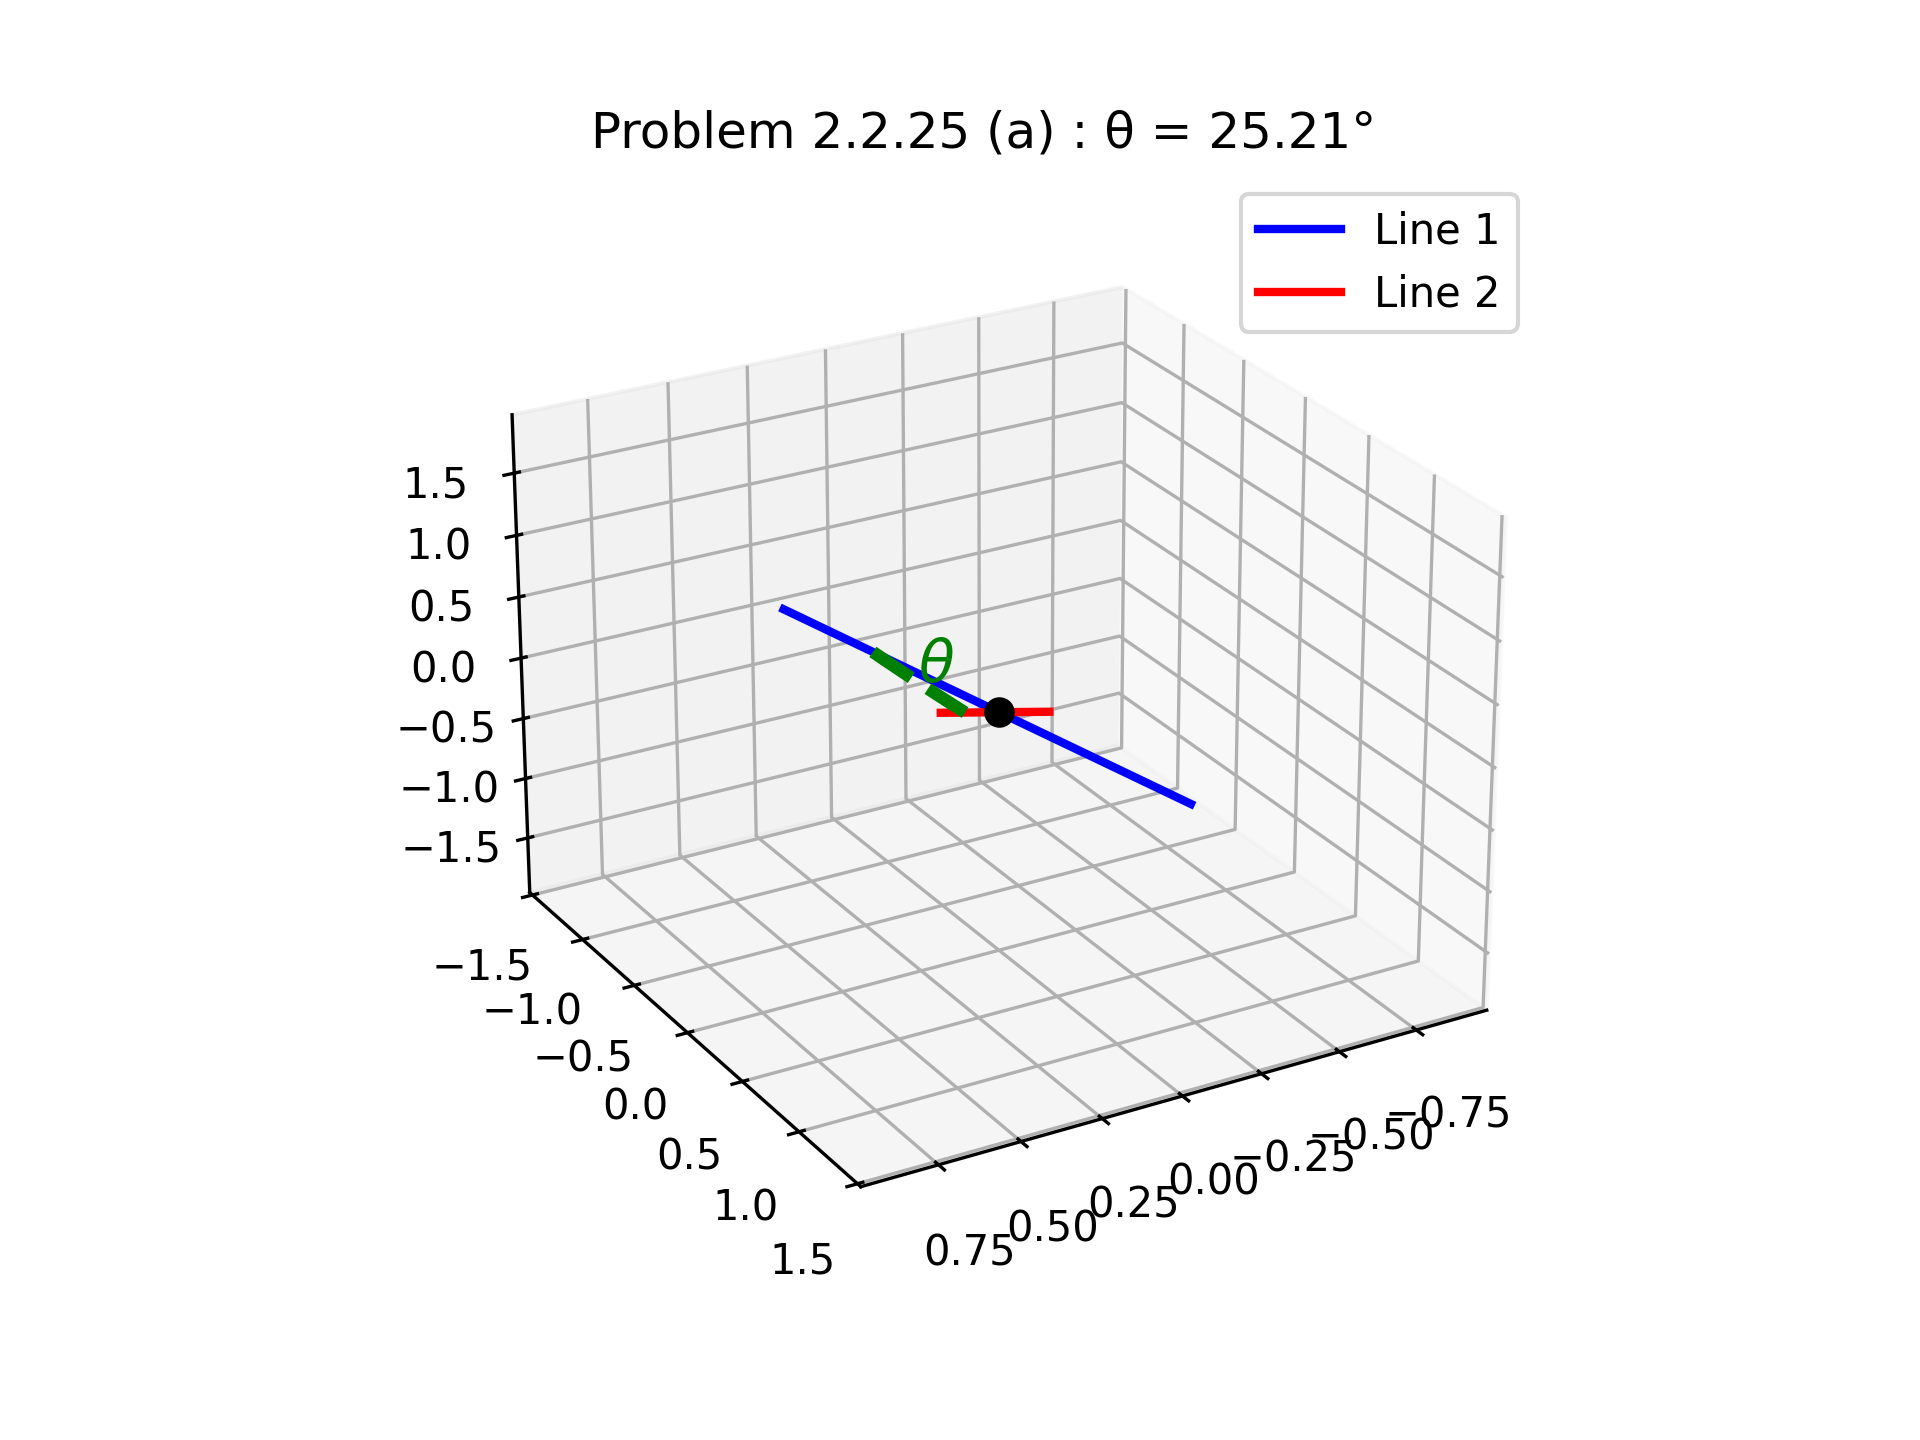
\includegraphics[width=0.9\columnwidth]{figs/figure_a.png}
    \caption{}
    \label{fig:placeholder}
\end{figure}
\end{frame}

\begin{frame}
    \frametitle{Plot}
\begin{figure}[H]
    \centering
    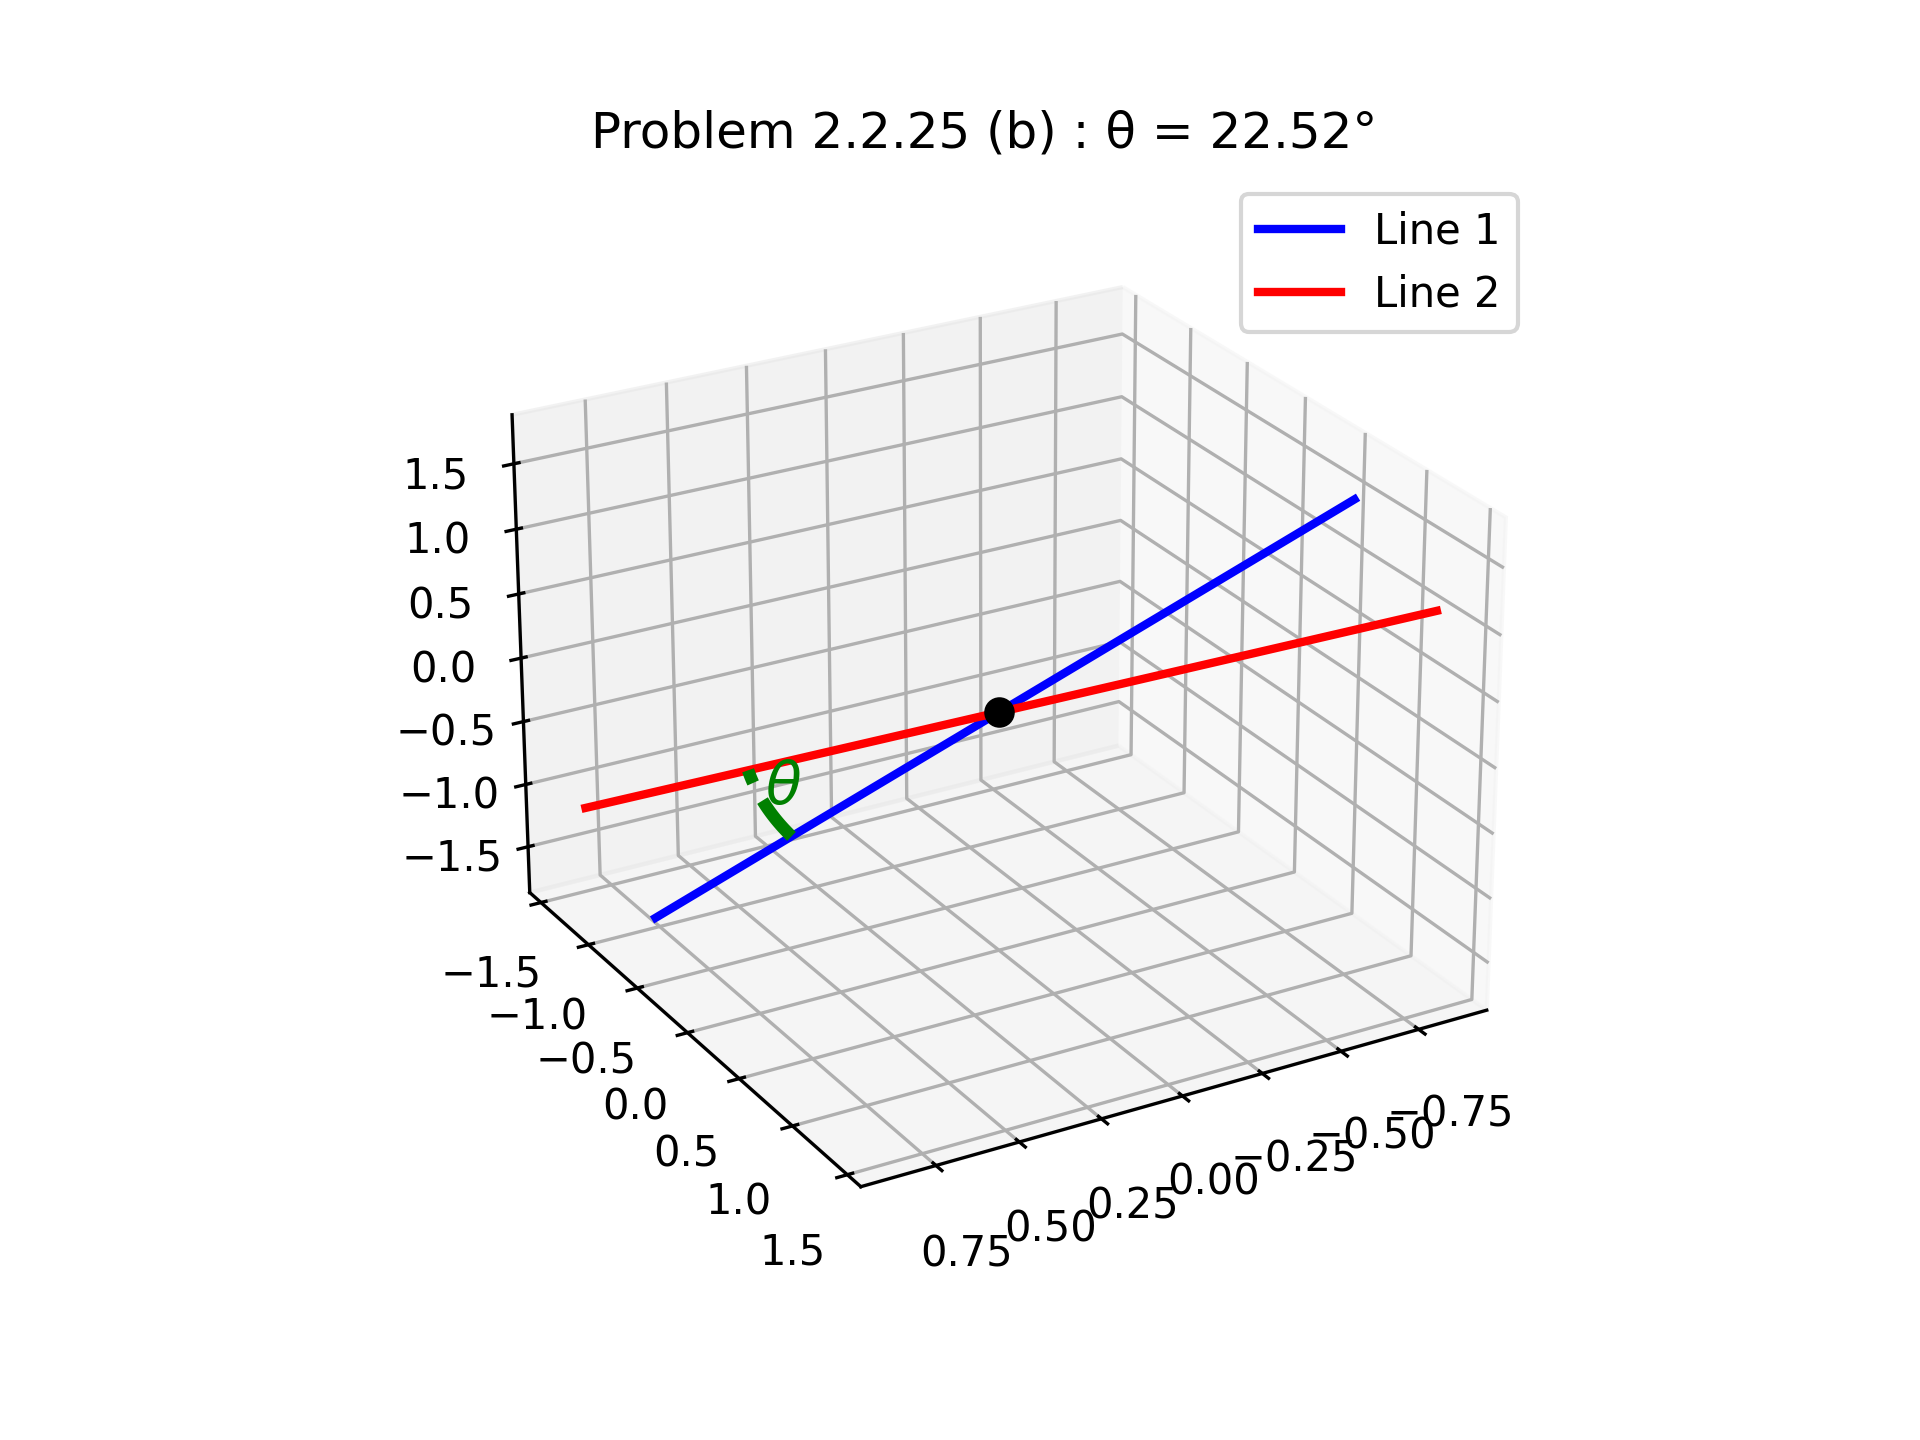
\includegraphics[width=0.9\columnwidth]{figs/figure_b.png}
    \caption{}
    \label{fig:placeholder}
\end{figure}
\end{frame}

\begin{frame}
    \frametitle{Plot}
\begin{figure}[H]
    \centering
    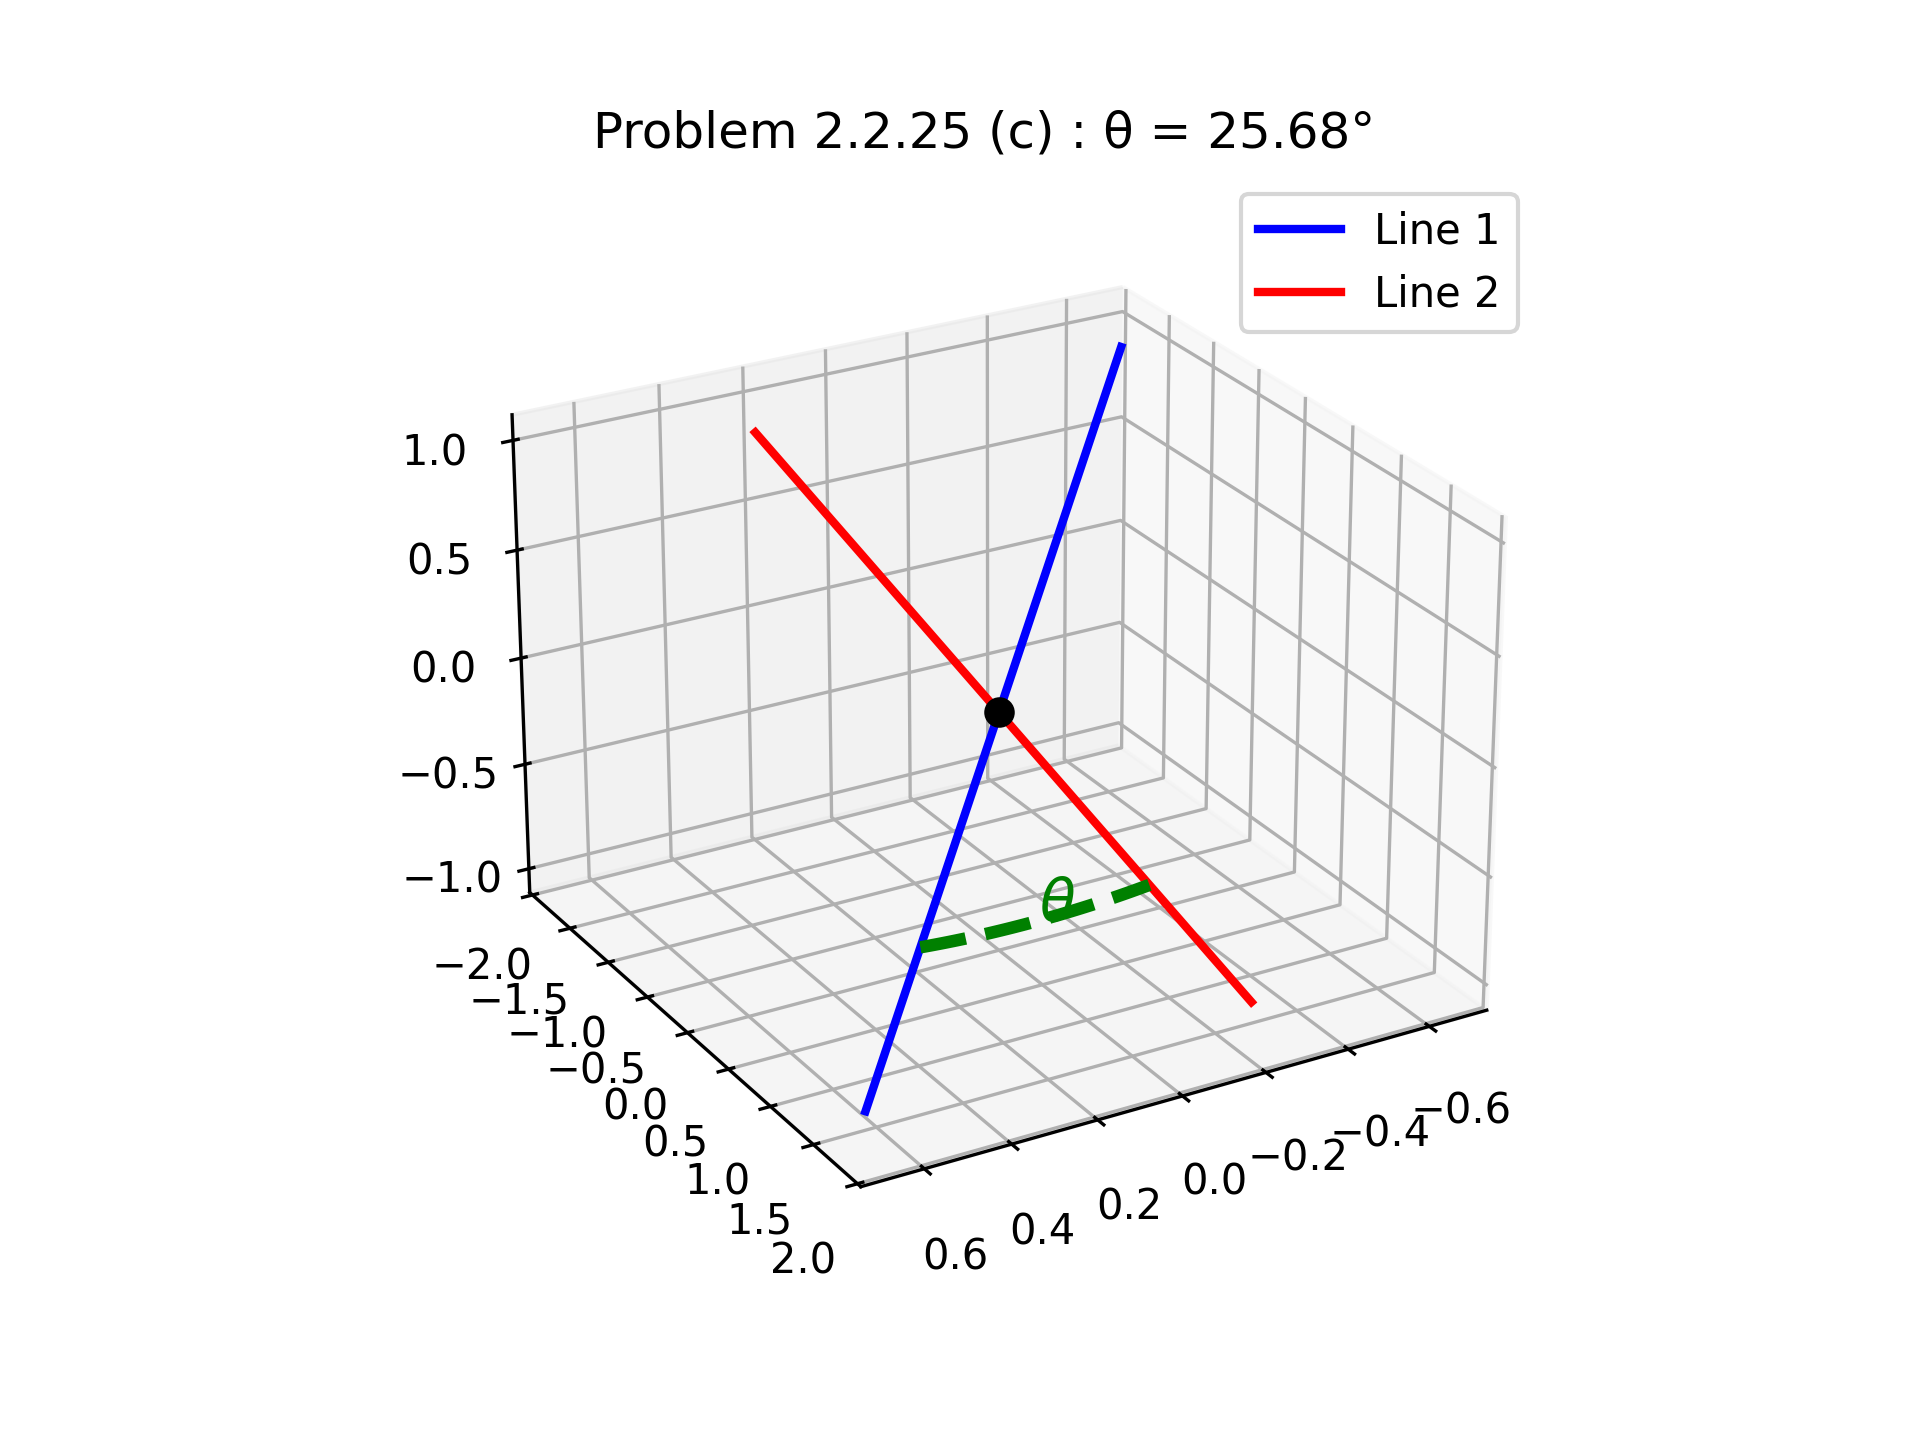
\includegraphics[width=0.9\columnwidth]{figs/figure_c.png}
    \caption{}
    \label{fig:placeholder}
\end{figure}
\end{frame}

\begin{frame}
    \frametitle{Plot}
\begin{figure}[H]
    \centering
    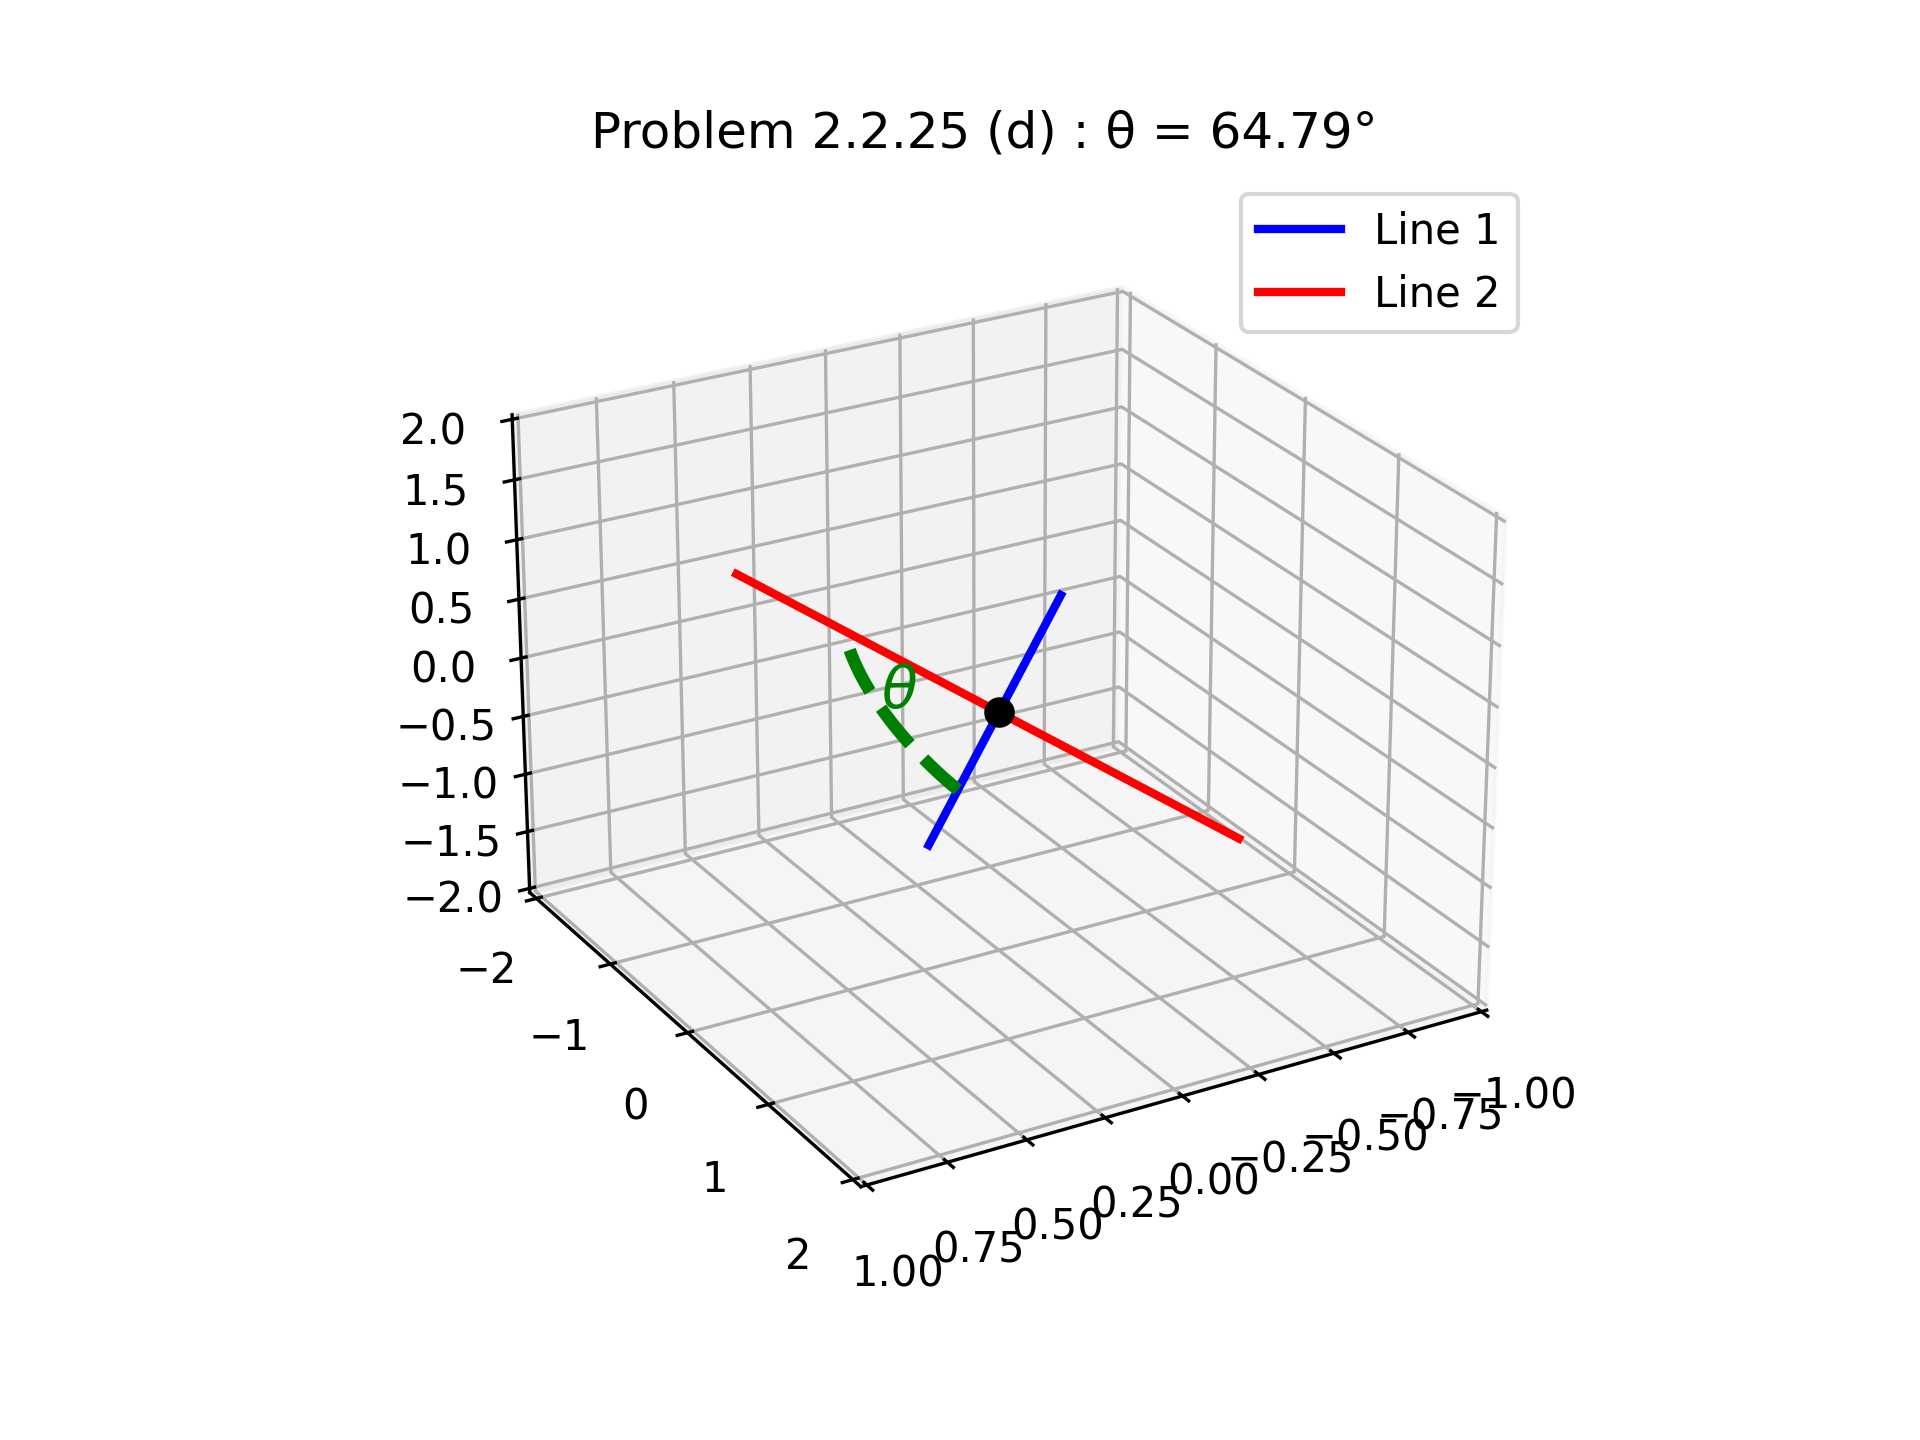
\includegraphics[width=0.9\columnwidth]{figs/figure_d.png}
    \caption{}
    \label{fig:placeholder}
\end{figure}
\end{frame}

\begin{frame}[fragile]
    \frametitle{Code - C}
    \begin{lstlisting}

#include <math.h>

// Function to compute angle in DEGREES between two vectors
double compute_angle_deg(double d1[3], double d2[3]) {
    // Dot product (matrix multiplication style)
    double dot = d1[0]*d2[0] + d1[1]*d2[1] + d1[2]*d2[2];

    // Norms
    double norm1 = sqrt(d1[0]*d1[0] + d1[1]*d1[1] + d1[2]*d1[2]);
    double norm2 = sqrt(d2[0]*d2[0] + d2[1]*d2[1] + d2[2]*d2[2]);

    // cos(theta)
    double cos_theta = dot / (norm1 * norm2);

\end{lstlisting}
\end{frame}

\begin{frame}[fragile]
    \frametitle{Code - C}
    \begin{lstlisting}


    // Clamp for numerical safety
    if (cos_theta > 1.0) cos_theta = 1.0;
    if (cos_theta < -1.0) cos_theta = -1.0;

    // Return angle in degrees
    return acos(cos_theta) * (180.0 / M_PI);
}



\end{lstlisting}
\end{frame}

\begin{frame}[fragile]
    \frametitle{Code - Python(with shared C code)}
    The code to obtain the required plot is
    \begin{lstlisting}
import numpy as np
import matplotlib.pyplot as plt
import ctypes

# Load C shared library
lib = ctypes.CDLL("./libangle.so")
lib.compute_angle_deg.restype = ctypes.c_double

def compute_angle_deg(d1, d2):
    arr1 = (ctypes.c_double * 3)(*d1)
    arr2 = (ctypes.c_double * 3)(*d2)
    return lib.compute_angle_deg(arr1, arr2)



\end{lstlisting}
\end{frame}
\begin{frame}[fragile]
\frametitle{Code - Python(with shared C code)}
\begin{lstlisting}

# All 4 cases of Problem 2.2.25
cases = [
    (np.array([3, 2, 6]), np.array([1, 2, 2]), "a"),
    (np.array([1, -1, -2]), np.array([3, -5, -4]), "b"),
    (np.array([2, 5, -3]), np.array([-1, 8, -4]), "c"),
    (np.array([2, 5, 1]), np.array([4, 1, 8]), "d")
]

for d1, d2, label in cases:
    theta_deg = compute_angle_deg(d1, d2)
    theta = np.radians(theta_deg)

    # Normalize vectors for visualization
    d1 = d1 / np.linalg.norm(d1)
    d2 = d2 / np.linalg.norm(d2)


\end{lstlisting}
\end{frame}

\begin{frame}[fragile]
\frametitle{Code - Python(with shared C code)}
\begin{lstlisting}
    # Generate line points (shorter range for clarity)
    t = np.linspace(-2, 2, 100)
    line1 = np.outer(t, d1)
    line2 = np.outer(t, d2)
    
    # Construct orthonormal basis in plane of d1, d2
    u1 = d1
    u2 = d2 - (d2 @ u1) * u1
    if np.linalg.norm(u2) > 1e-8:
        u2 /= np.linalg.norm(u2)
    
    # Arc between d1 and d2
    arc_t = np.linspace(0, theta, 50)
    arc_points = np.array([np.cos(a)*u1 + np.sin(a)*u2 for a in arc_t]) * 1.2


\end{lstlisting}
\end{frame}

\begin{frame}[fragile]
\frametitle{Code - Python(with shared C code)}
\begin{lstlisting}
    # Plot
    fig = plt.figure()
    ax = fig.add_subplot(111, projection='3d')
    ax.plot(line1[:,0], line1[:,1], line1[:,2], color="blue", label="Line 1", lw=2)
    ax.plot(line2[:,0], line2[:,1], line2[:,2], color="red", label="Line 2", lw=2)
    ax.plot(arc_points[:,0], arc_points[:,1], arc_points[:,2],
            color="green", lw=3, ls="--")
    
    # Label $\theta$ near the arc
    mid = arc_points[len(arc_points)//2]
    ax.text(mid[0], mid[1], mid[2], r"$\theta$", fontsize=14, color="green")
    
    # Origin
    ax.scatter(0, 0, 0, color="black", s=40)


\end{lstlisting}
\end{frame}

\begin{frame}[fragile]
\frametitle{Code - Python(with shared C code)}
\begin{lstlisting}
    # Titles
    ax.set_title(f"Problem 2.2.25 ({label}) : theta = {theta_deg:.2f}")
    ax.legend()
    
    # Set fixed camera view for clarity
    ax.view_init(elev=25, azim=60)
    
    # Save & show
    plt.savefig(f"figure_{label}.png", dpi=300)
    plt.show()


\end{lstlisting}
\end{frame}


\begin{frame}[fragile]
\frametitle{Code - Python only}
\begin{lstlisting}

import numpy as np
import matplotlib.pyplot as plt

# All 4 cases of Problem 2.2.25
cases = [
    (np.array([3, 2, 6]), np.array([1, 2, 2]), "a"),
    (np.array([1, -1, -2]), np.array([3, -5, -4]), "b"),
    (np.array([2, 5, -3]), np.array([-1, 8, -4]), "c"),
    (np.array([2, 5, 1]), np.array([4, 1, 8]), "d")
]

# Print table header
print("Problem2.2.25-Angles-between-lines")
print("-------------------------------------")



\end{lstlisting}
\end{frame}
\begin{frame}[fragile]
\frametitle{Code - Python only}
\begin{lstlisting}
for d1, d2, label in cases:
    # Compute angle using numpy
    cos_theta = (d1 @ d2) / (np.linalg.norm(d1) * np.linalg.norm(d2))
    cos_theta = np.clip(cos_theta, -1.0, 1.0)  # numerical safety
    theta = np.arccos(cos_theta)
    theta_deg = np.degrees(theta)

    # Print result in terminal
    print(f"Case ({label}): \theta = {theta_deg:.2f}")

    # Normalize for visualization
    d1 = d1 / np.linalg.norm(d1)
    d2 = d2 / np.linalg.norm(d2)




\end{lstlisting}
\end{frame}

\begin{frame}[fragile]
\frametitle{Code - Python only}
\begin{lstlisting}
    # Generate shorter line segments
    t = np.linspace(-2, 2, 100)
    line1 = np.outer(t, d1)
    line2 = np.outer(t, d2)

    # Orthonormal basis for arc
    u1 = d1
    u2 = d2 - (d2 @ u1) * u1
    if np.linalg.norm(u2) > 1e-8:
        u2 /= np.linalg.norm(u2)

    # Arc between d1 and d2
    arc_t = np.linspace(0, theta, 50)
    arc_points = np.array([np.cos(a)*u1 + np.sin(a)*u2 for a in arc_t]) * 1.2



\end{lstlisting}
\end{frame}

\begin{frame}[fragile]
\frametitle{Code - Python only}
\begin{lstlisting}
    # Plot
    fig = plt.figure()
    ax = fig.add_subplot(111, projection='3d')
    ax.plot(line1[:,0], line1[:,1], line1[:,2], color="blue", label="Line 1", lw=2)
    ax.plot(line2[:,0], line2[:,1], line2[:,2], color="red", label="Line 2", lw=2)
    ax.plot(arc_points[:,0], arc_points[:,1], arc_points[:,2],
            color="green", lw=3, ls="--")

    # Label $\theta$
    mid = arc_points[len(arc_points)//2]
    ax.text(mid[0], mid[1], mid[2], r"$\theta$", fontsize=14, color="green")

    # Origin
    ax.scatter(0, 0, 0, color="black", s=40)



\end{lstlisting}
\end{frame}

\begin{frame}[fragile]
\frametitle{Code - Python only}
\begin{lstlisting}
    # Title
    ax.set_title(f"Problem 2.2.25 ({label}) : \theta = {theta_deg:.2f}")
    ax.legend()

    # Adjust camera view
    ax.view_init(elev=25, azim=60)

    # Save and show
    plt.savefig(f"/sdcard/ee1030-2025/ai25btech11032/Matgeo/2.2.25/figs/newfigure_{label}_python.png", dpi=300)
    plt.show()



\end{lstlisting}
\end{frame}

\end{document}

